
\documentclass{article}

\usepackage[margin=1in]{geometry}
\linespread{1.2}

\usepackage{graphicx}
\usepackage{amsfonts}
\usepackage{amsmath}
\usepackage{authblk}
\usepackage{tikz}\usetikzlibrary{decorations.pathmorphing}
%\usepackage[style=authoryear]{biblatex}
\usepackage{natbib}
\bibliographystyle{../apa-good}
%\addbibresource{journal-article.bib}

\title{Swinging, Fast and Slow:\\Interpreting variation in baseball swing tracking metrics}
\author[1]{Scott Powers}
\author[2]{Ronald Yurko}
\affil[1]{Department of Sport Management, Rice University}
\affil[2]{Department of Statistics \& Data Science, Carnegie Mellon University}

\begin{document}

  \maketitle
	
  \begin{abstract}
    The abstract goes here.
  \end{abstract}

  \section{Introduction}
  \label{sec:introduction}

    \begin{figure}
      \centering
      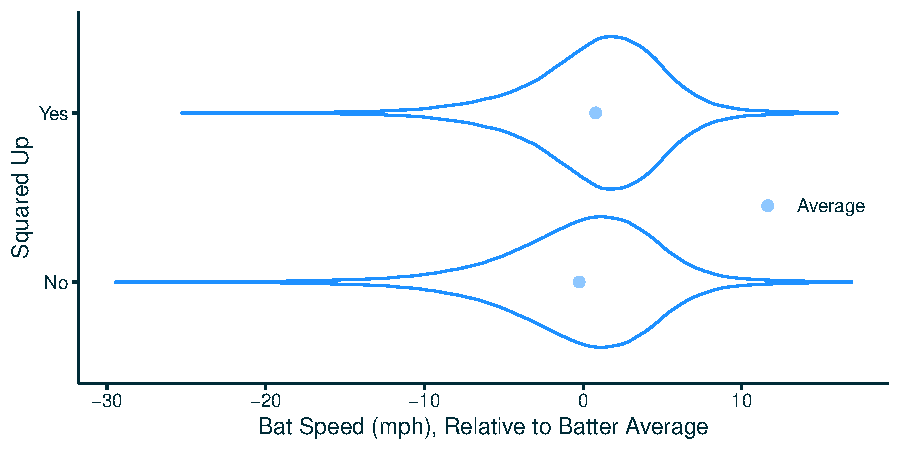
\includegraphics[width = 0.8\textwidth]{../../figures/counterintuitive.pdf}
      \caption{\it Distribution of bat speed relative to batter average by contact quality (squared up or not), across all swings in the dataset. The x-axis represents the difference between the bat speed and the batter's average bat speed. Following MLB's definition, a swing is considered ``squared up'' if the batted ball's exit velocity is at least 80\% of the theoretical maximum (given pitch speed and bat speed), a proxy for good contact.}
      \label{fig:counterintuitive}
    \end{figure}

    \begin{figure}
      \centering
      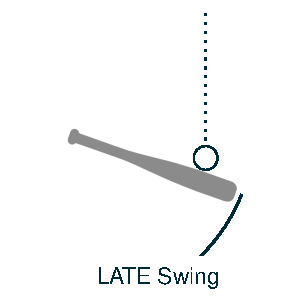
\includegraphics[width = 0.4\textwidth]{../../figures/swing_late.pdf}
      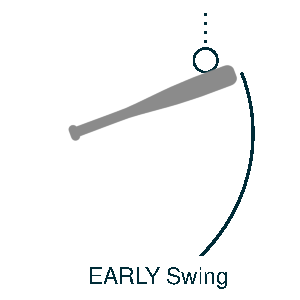
\includegraphics[width = 0.4\textwidth]{../../figures/swing_early.pdf}
      \caption{\it A diagram illustrating the effect of swing timing on swing length measurement due to the fact that swing length is measured at the point of contact. Imagining two swings with the exact same mechanics, the left image shows the swing length measurement if the swing is late, and the right image shows the swing length measurement if the swing is early.}
      \label{fig:swing-diagram}
    \end{figure}

    \subsection{Related Work}
    \label{sec:related-work}

  \section{Data}
  \label{sec:data}

  \section{Methods}
  \label{sec:methods}

    \subsection{Intention Model}
    \label{sec:methods-intention}

    \subsection{Causal Model}
    \label{sec:methods-causal}

  \section{Results}
  \label{sec:results}

    \subsection{Intention Model}
    \label{sec:results-intention}

      \begin{figure}
        \centering
        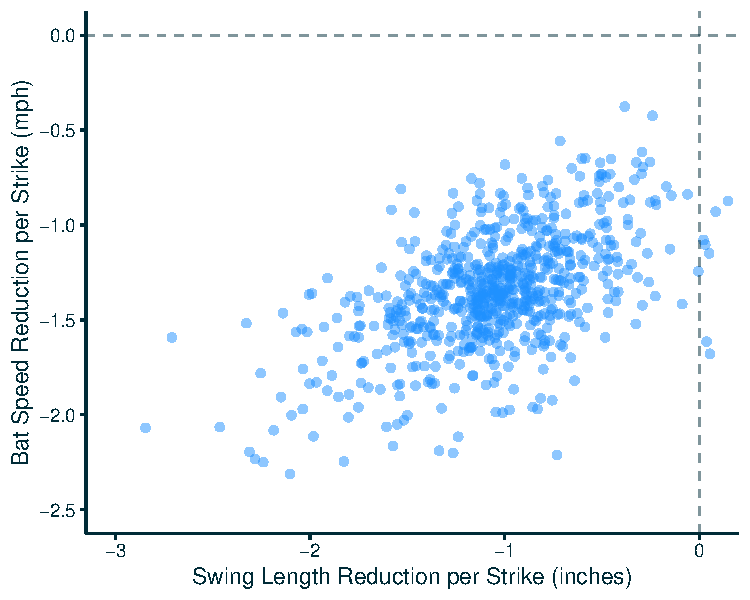
\includegraphics[width = 0.6\textwidth]{../../figures/approach.pdf}
        \caption{\it Estimated batter random slopes for strikes in the intention model. Each point is a batter $b$, with the x-value representing $\hat\beta^S + \hat\gamma^S_b$ from the model (\ref{eqn:intention-swing-length}) and the y-value representing the same quantity from the model (\ref{eqn:intention-bat-speed}). This quantity is interpretable as the expected change in swing length (or bat speed) corresponding to a one-strike increase in the ball-strike count.}
        \label{fig:approach}
      \end{figure}

    \subsection{Causal Model}
    \label{sec:results-causal}

      \begin{figure}
        \centering
        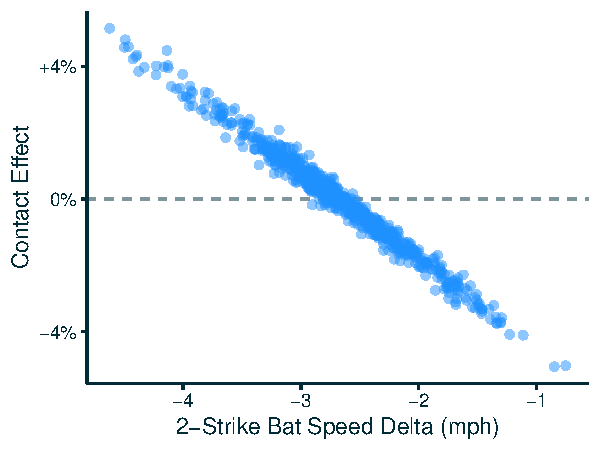
\includegraphics[width = 0.49\textwidth]{../../figures/bat_speed_contact.pdf}
        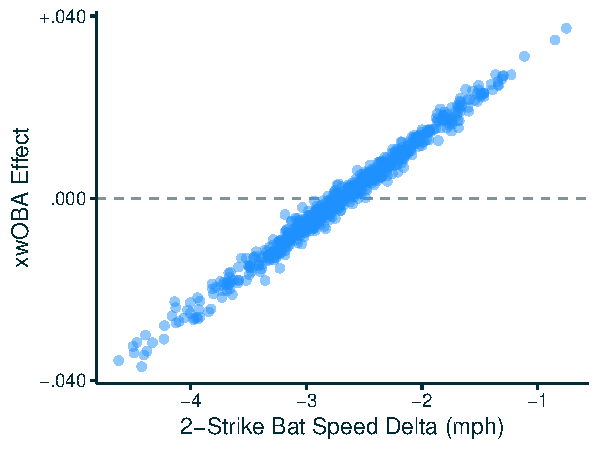
\includegraphics[width = 0.49\textwidth]{../../figures/bat_speed_power.pdf}
        \caption{\it Estimated causal effect of bat speed on contact (left) and power (right). Each point is a batter; the x-axis shows how much the batter slows their swing in two-strike counts, relative to zero-strike counts, from the model (\ref{eqn:intention-bat-speed}); the y-axis shows the estimated combined effect of the batter's bat speed and swing length adjustments on contact rate (left) and xwOBAcon (right) in two-strike counts, from the model (\ref{eqn:causal}). Contact rate is the percentage of swings contacting the ball, and xwOBAcon is a standard sabermetric statistic for measuring power. Its units are runs per plate appearance.}
        \label{fig:results-causal}
      \end{figure}

      \begin{figure}
        \centering
        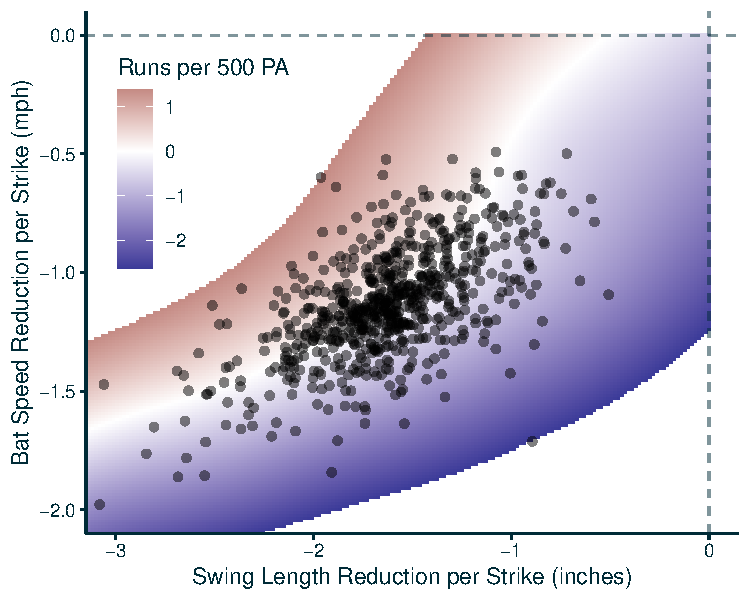
\includegraphics[width = 0.8\textwidth]{../../figures/approach_run_value.pdf}
        \caption{\it Estimated causal effect of batters' approaches, measured on the scale of runs per 500 plate appearances (PA). This figure shows the same data as Figure \ref{fig:approach} except that the background gradient reports the estimated run value of each approach. If an approach is valued at z runs, the interpretation is that the average batter with this approach is expected to produce z runs more than if they adopted an average approach, as measured by linear weights.}
        \label{fig:approach-run-value}
      \end{figure}

    \subsection{Other Sources of Swing Variation}
    \label{sec:results-other}

      \begin{figure}
        \centering
        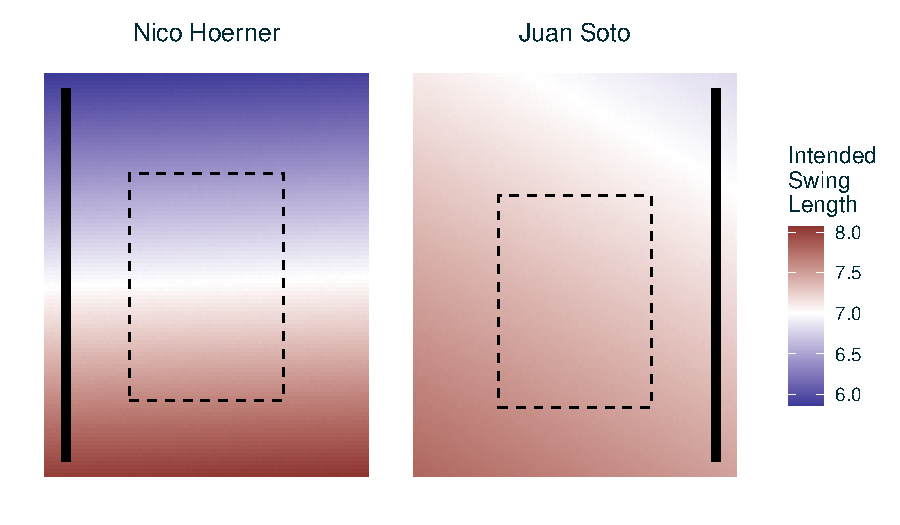
\includegraphics[width = 0.8\textwidth]{../../figures/adaptation.pdf}
        \caption{\it Expected swing length by pitch location for two sample batters: Nico Hoerner (left) and Juan Soto (right), from the perspective of behind home plate. The thick vertical bars show the side of the plate on which the batter stands, and the dashed rectangle shows the strike zone, which depends on the height and stance of the batter. The color shows the predicted swing length  from model (\ref{eqn:intention-swing-length}) assuming a 0-0 count.}
        \label{fig:adaptation}
      \end{figure}

  \section{Discussion}
  \label{sec:discussion}

  \bibliography{../swingfastslow}

\end{document}